\documentclass[11pt]{article}
\usepackage[hmargin=1in,vmargin=1in]{geometry}
\usepackage[document]{ragged2e}
\usepackage{xcolor}
\usepackage{amsmath,amssymb,amsfonts,url,sectsty,framed,tcolorbox,framed}
\usepackage{tikz}
\usepackage{nicematrix}
\newcommand{\pf}{{\bf Proof: }}
\newtheorem{theorem}{Theorem}
\newtheorem{lemma}{Lemma}
\newtheorem{proposition}{Proposition}
\newtheorem{definition}{Definition}
\newtheorem{remark}{Remark}
\newcommand{\qed}{\hfill \rule{2mm}{2mm}}


\begin{document}
%%%%%%%%%%%%%%%%%%%%%%%%%%%%%%%%%%%%%%%%%%%%%%%%%%%%%%%%%%%%%%%%%%%%%
\noindent
\rule{\textwidth}{1pt}
\begin{center}
{\bf [CS304] Introduction to Cryptography and Network Security}
\end{center}
Course Instructor: Dr. Dibyendu Roy \hfill Winter 2022-2023\\
Scribed by: Chitranshi Srivastava (202051055) \hfill Lecture 7 (Week \#4)
\\
\rule{\textwidth}{1pt}
%%%%%%%%%%%%%%%%%%%%%%%%%%%%%%%%%%%%%%%%%%%%%%%%%%%%%%%%%%%
%write here
In the previous week, we discussed about Data Encryption Standard(DES) - its encryption, decryption and its complementarity property.

\section{Attack Models}
\subsection{Cipher Text only Attack}
Here, the attacker only knows the cipher text generated by an algorithm. The algorithm is known to everyone. The goal is to recover the corresponding plain text or find the secret key. If any of this is recovered, then the cipher is said to be broken. But if some part of plain text is recovered due to randomness, then the cipher is not said to be broken.

\subsection{Known Plain text Attack}
Here, the attacker knows some part of the plain text corresponding to the cipher text. Let's suppose that the attacker knows plain text $p_1, p_2,....p_n$ corresponding to the cipher text $c_1, c_2,...., c_n$. The goal here is to generate new plain text-cipher text pair, for example, new plain text $p$ from new cipher text $c$, such that $c \notin \{c_1, c_2,...., c_n\}$ or to recover the secret key.\\
\vspace{3mm}
The attacker has the advantage of knowing some plain text corresponding to cipher text. The Known Plain Text Attack is therefore stronger than Cipher Text Only Attack. If an encryption algorithm is secure to Known Plain Text Attack, then it will surely be secure for Cipher Text only Attack, but the reverse is not true.

\subsection{Chosen Plain text Attack}
Here, the attacker chooses the plain text according to his/her choice and he/she will be provided with the corresponding cipher text using the encryption algorithm. From this, the attacker tries to find the plain text for some different cipher text or tries to recover the secret key.\\
\vspace{3mm}
This attack model is much stronger than the Known Plain Text Attack as the attacker has the freedom to select the plain text arbitrarily. Hence, any encryption algorithm that is secure under this model, is also secure under the other two attack models.

\subsection{Chosen Cipher text Attack}
In this attack model, the attacker chooses some cipher text and is allowed to get the corresponding plain text. The goal of the attack is to get some new cipher text-plain text pair or recovering the secret key.\\
\vspace{3mm}
These attacks are much stronger in the Public-Key cryptography domains, as the key used to decrypt will be receiver's secret key. Hence, the attacker, if successful, will get the receiver's secret key.


\section{Cryptanalysis of DES}
DES provides 56 bit security. The parity bits are generated using these 56 bits, so they are not taken into consideration here.This means that a Brute Force Attack or Exhaustive Search on DES will look for $2^{56}$ keys to get the secret key.\\
This search space can be reduced to $2^{55}$ keys using the complementation property of DES.
\vspace{3mm}
The complementation property states:
\begin{center}
    $DES(M, K) = C$\\
    $DES(\overline{M}, \overline{K}) = \overline{C}$
\end{center}
Let's now consider the Chosen Plain Text Attack Model. The attacker chooses two plain texts $M$ and $\overline{M}$ and asks for cipher text corresponding to these plain texts. Lets say:
\begin{center}
    $DES(M, K) = C_1$\\
    $DES(\overline{M}, K) = C_2$
\end{center}
Attacker is getting $C_1$ and $C_2$ and his/her goal is to get the secret key $K$. 
\vspace{3mm}
We know about the complementation property of DES. So we perform the operation:
\begin{center}
    $DES(\overline{\overline{M}}, \overline{K}) = \overline{C_2}$\\
    \vspace{1mm}
    $\implies DES(M, \overline{K}) = \overline{C_2}$
\end{center}
Now, the attacker has the following information:
\begin{center}
    $DES(M, K) = C_1$\\
    \vspace{1mm}
    $DES(M, \overline{K}) = \overline{C_2}$
\end{center}
where, $C_1, C_2$ and hence $\overline{C_2}$ are known to attacker. \\
The set of all possible keys using 56 bits, is as follows:
\begin{center}
    $keys = \{K_1, K_2,...., K_{2^{56}}\}$
\end{center}
Attacker chooses a key, say $K_i \in keys$. Now, the attacker performs the following:
\begin{center}
    $DES(M, K_i) = \Tilde{C}$
\end{center}
Now, from the information that we have, we can have the following interpretations:
\begin{center}
    if $\Tilde{C} = C_1 \implies K_i = K$(the actual secret key)\\
    \vspace{1mm}
    if $\Tilde{C} = \overline{C_2} \implies K_i = \overline{K}$(complement of actual key)\\
    \vspace{1mm}
    if $\Tilde{C} \neq C_1 \implies K_i \neq K$\\
    \vspace{1mm}
    if $\Tilde{C} \neq \overline{C_2} \implies K_i \neq \overline{K} \implies \overline{K_i} \neq K$
\end{center}
Hence, for each key $K_i$, either the actual key $K$ will be found, or we will be able to eliminate two keys, $K_i$ and $\overline{K_i}$. 
\\
Hence, our search space has become half and we need to search for $2^{55}$ keys to get the actual key.\\
\vspace{5mm}
DES is vulnerable to  different attacks such as Differential Attacks and Linearization Attacks. It has been observed that DES can be broken in approximately $2^{43}$ complexity. \\
One possible solution is to increase the length of the secret key;increase the length of the secret key to $n$ times and perform the encryption $n$ times.

\section{Double Encryption of DES}
The message is encrypted twice using the DES algorithm. The encryption and decryption function remains same. The length of the secret key is 112 bits and is as follows:
\begin{center}
    $K = K_1 || K_2$
\end{center}
\vspace{3mm}
One way to do double encryption is :
\begin{center}
    \tikzset{every picture/.style={line width=0.75pt}} 
    
    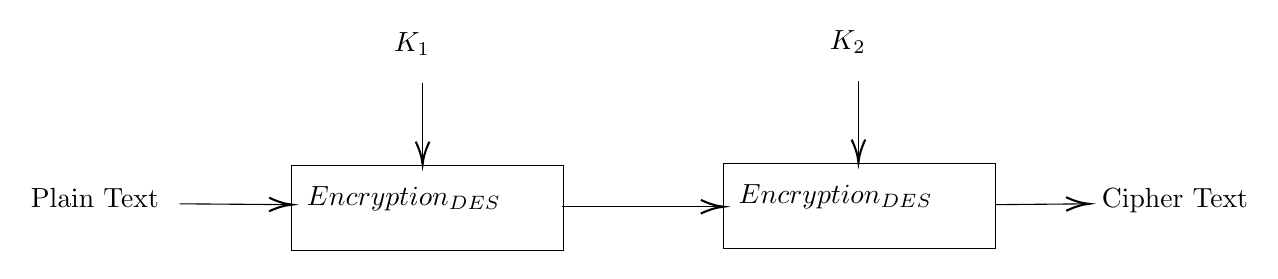
\begin{tikzpicture}[x=0.75pt,y=0.75pt,yscale=-1,xscale=1]
    
        \draw   (163,100) -- (294,100) -- (294,141) -- (163,141) -- cycle ;
        \draw   (371,99) -- (502,99) -- (502,140) -- (371,140) -- cycle ;
        \draw    (109,118.6) -- (161,118.99) ;
        \draw [shift={(163,119)}, rotate = 180.42] [color={rgb, 255:red, 0; green, 0; blue, 0 }  ][line width=0.75]    (10.93,-3.29) .. controls (6.95,-1.4) and (3.31,-0.3) .. (0,0) .. controls (3.31,0.3) and (6.95,1.4) .. (10.93,3.29)   ;
        \draw    (293,120) -- (369,120) ;
        \draw [shift={(371,120)}, rotate = 180] [color={rgb, 255:red, 0; green, 0; blue, 0 }  ][line width=0.75]    (10.93,-3.29) .. controls (6.95,-1.4) and (3.31,-0.3) .. (0,0) .. controls (3.31,0.3) and (6.95,1.4) .. (10.93,3.29)   ;
        \draw    (502,119) -- (545,118.62) ;
        \draw [shift={(547,118.6)}, rotate = 179.49] [color={rgb, 255:red, 0; green, 0; blue, 0 }  ][line width=0.75]    (10.93,-3.29) .. controls (6.95,-1.4) and (3.31,-0.3) .. (0,0) .. controls (3.31,0.3) and (6.95,1.4) .. (10.93,3.29)   ;
        \draw    (226,60.6) -- (226,97.6) ;
        \draw [shift={(226,99.6)}, rotate = 270] [color={rgb, 255:red, 0; green, 0; blue, 0 }  ][line width=0.75]    (10.93,-3.29) .. controls (6.95,-1.4) and (3.31,-0.3) .. (0,0) .. controls (3.31,0.3) and (6.95,1.4) .. (10.93,3.29)   ;
        \draw    (436,59.6) -- (436,96.6) ;
        \draw [shift={(436,98.6)}, rotate = 270] [color={rgb, 255:red, 0; green, 0; blue, 0 }  ][line width=0.75]    (10.93,-3.29) .. controls (6.95,-1.4) and (3.31,-0.3) .. (0,0) .. controls (3.31,0.3) and (6.95,1.4) .. (10.93,3.29)   ;
        
        \draw (169,109) node [anchor=north west][inner sep=0.75pt]   [align=left] {$Encryption_{DES}$};
        \draw (377,108) node [anchor=north west][inner sep=0.75pt]   [align=left] {$Encryption_{DES}$};
        \draw (36,110) node [anchor=north west][inner sep=0.75pt]   [align=left] {Plain Text};
        \draw (552,110) node [anchor=north west][inner sep=0.75pt]   [align=left] {Cipher Text};
        \draw (211,35) node [anchor=north west][inner sep=0.75pt]   [align=left] {$K_1$};
        \draw (421,34) node [anchor=north west][inner sep=0.75pt]   [align=left] {$K_2$};
    
    \end{tikzpicture}
    \textbf{Encryption}
    \vspace{3mm}
    
    \tikzset{every picture/.style={line width=0.75pt}}     
    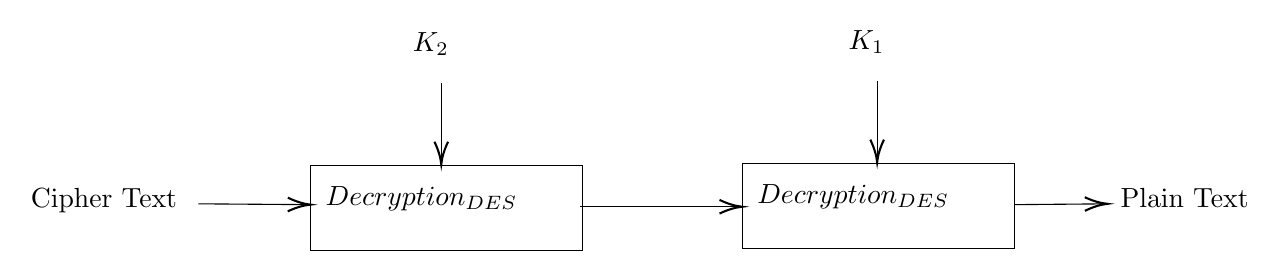
\begin{tikzpicture}[x=0.75pt,y=0.75pt,yscale=-1,xscale=1]
    

        \draw   (166,231) -- (297,231) -- (297,272) -- (166,272) -- cycle ;
        \draw   (374,230) -- (505,230) -- (505,271) -- (374,271) -- cycle ; 
        \draw    (112,249.6) -- (164,249.99) ;
        \draw [shift={(166,250)}, rotate = 180.42] [color={rgb, 255:red, 0; green, 0; blue, 0 }  ][line width=0.75]    (10.93,-3.29) .. controls (6.95,-1.4) and (3.31,-0.3) .. (0,0) .. controls (3.31,0.3) and (6.95,1.4) .. (10.93,3.29)   ; 
        \draw    (296,251) -- (372,251) ;
        \draw [shift={(374,251)}, rotate = 180] [color={rgb, 255:red, 0; green, 0; blue, 0 }  ][line width=0.75]    (10.93,-3.29) .. controls (6.95,-1.4) and (3.31,-0.3) .. (0,0) .. controls (3.31,0.3) and (6.95,1.4) .. (10.93,3.29)   ; 
        \draw    (505,250) -- (548,249.62) ;
        \draw [shift={(550,249.6)}, rotate = 179.49] [color={rgb, 255:red, 0; green, 0; blue, 0 }  ][line width=0.75]    (10.93,-3.29) .. controls (6.95,-1.4) and (3.31,-0.3) .. (0,0) .. controls (3.31,0.3) and (6.95,1.4) .. (10.93,3.29)   ; 
        \draw    (229,191.6) -- (229,228.6) ;
        \draw [shift={(229,230.6)}, rotate = 270] [color={rgb, 255:red, 0; green, 0; blue, 0 }  ][line width=0.75]    (10.93,-3.29) .. controls (6.95,-1.4) and (3.31,-0.3) .. (0,0) .. controls (3.31,0.3) and (6.95,1.4) .. (10.93,3.29)   ; 
        \draw    (439,190.6) -- (439,227.6) ;
        \draw [shift={(439,229.6)}, rotate = 270] [color={rgb, 255:red, 0; green, 0; blue, 0 }  ][line width=0.75]    (10.93,-3.29) .. controls (6.95,-1.4) and (3.31,-0.3) .. (0,0) .. controls (3.31,0.3) and (6.95,1.4) .. (10.93,3.29)   ;
        
        \draw (172,240) node [anchor=north west][inner sep=0.75pt]   [align=left] {$Decryption_{DES}$};
        \draw (380,239) node [anchor=north west][inner sep=0.75pt]   [align=left] {$Decryption_{DES}$};
        \draw (30,241) node [anchor=north west][inner sep=0.75pt]   [align=left] {Cipher Text};
        \draw (555,241) node [anchor=north west][inner sep=0.75pt]   [align=left] {Plain Text};
        \draw (214,166) node [anchor=north west][inner sep=0.75pt]   [align=left] {$K_2$};
        \draw (424,165) node [anchor=north west][inner sep=0.75pt]   [align=left] {$K_1$};
    \end{tikzpicture}

    \textbf{Decryption}
\end{center}
\textbf{Encryption:}\\
We first encrypt using key $K_1$ and then with key $K_2$.\\
\textbf{Decryption:}\\
We first encrypt using key $K_2$ and then with key $K_1$.\\
\vspace{5mm}
We can use different permutations of Encryption and Decryption functions of the basic DES implementation like above. Another example is:
\begin{center}
    \tikzset{every picture/.style={line width=0.75pt}} 
    
    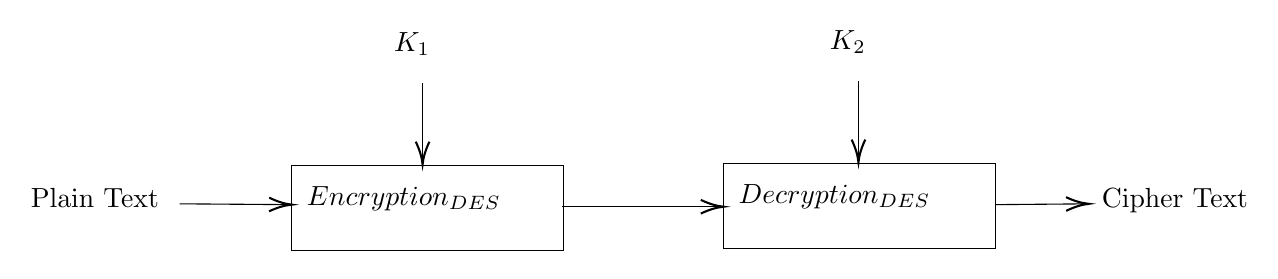
\begin{tikzpicture}[x=0.75pt,y=0.75pt,yscale=-1,xscale=1]
    
        \draw   (163,100) -- (294,100) -- (294,141) -- (163,141) -- cycle ;
        \draw   (371,99) -- (502,99) -- (502,140) -- (371,140) -- cycle ;
        \draw    (109,118.6) -- (161,118.99) ;
        \draw [shift={(163,119)}, rotate = 180.42] [color={rgb, 255:red, 0; green, 0; blue, 0 }  ][line width=0.75]    (10.93,-3.29) .. controls (6.95,-1.4) and (3.31,-0.3) .. (0,0) .. controls (3.31,0.3) and (6.95,1.4) .. (10.93,3.29)   ;
        \draw    (293,120) -- (369,120) ;
        \draw [shift={(371,120)}, rotate = 180] [color={rgb, 255:red, 0; green, 0; blue, 0 }  ][line width=0.75]    (10.93,-3.29) .. controls (6.95,-1.4) and (3.31,-0.3) .. (0,0) .. controls (3.31,0.3) and (6.95,1.4) .. (10.93,3.29)   ;
        \draw    (502,119) -- (545,118.62) ;
        \draw [shift={(547,118.6)}, rotate = 179.49] [color={rgb, 255:red, 0; green, 0; blue, 0 }  ][line width=0.75]    (10.93,-3.29) .. controls (6.95,-1.4) and (3.31,-0.3) .. (0,0) .. controls (3.31,0.3) and (6.95,1.4) .. (10.93,3.29)   ;
        \draw    (226,60.6) -- (226,97.6) ;
        \draw [shift={(226,99.6)}, rotate = 270] [color={rgb, 255:red, 0; green, 0; blue, 0 }  ][line width=0.75]    (10.93,-3.29) .. controls (6.95,-1.4) and (3.31,-0.3) .. (0,0) .. controls (3.31,0.3) and (6.95,1.4) .. (10.93,3.29)   ;
        \draw    (436,59.6) -- (436,96.6) ;
        \draw [shift={(436,98.6)}, rotate = 270] [color={rgb, 255:red, 0; green, 0; blue, 0 }  ][line width=0.75]    (10.93,-3.29) .. controls (6.95,-1.4) and (3.31,-0.3) .. (0,0) .. controls (3.31,0.3) and (6.95,1.4) .. (10.93,3.29)   ;
        
        \draw (169,109) node [anchor=north west][inner sep=0.75pt]   [align=left] {$Encryption_{DES}$};
        \draw (377,108) node [anchor=north west][inner sep=0.75pt]   [align=left] {$Decryption_{DES}$};
        \draw (36,110) node [anchor=north west][inner sep=0.75pt]   [align=left] {Plain Text};
        \draw (552,110) node [anchor=north west][inner sep=0.75pt]   [align=left] {Cipher Text};
        \draw (211,35) node [anchor=north west][inner sep=0.75pt]   [align=left] {$K_1$};
        \draw (421,34) node [anchor=north west][inner sep=0.75pt]   [align=left] {$K_2$};
    
    \end{tikzpicture}
    \textbf{Encryption}
    \vspace{3mm}
    
    \tikzset{every picture/.style={line width=0.75pt}}     
    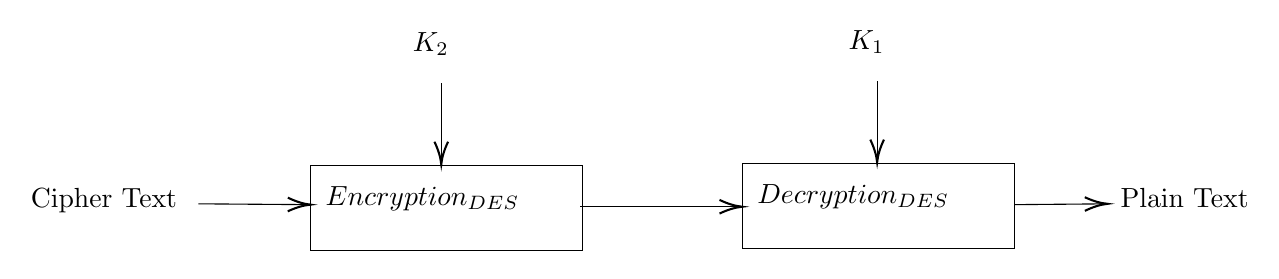
\begin{tikzpicture}[x=0.75pt,y=0.75pt,yscale=-1,xscale=1]
        \draw   (166,231) -- (297,231) -- (297,272) -- (166,272) -- cycle ;
        \draw   (374,230) -- (505,230) -- (505,271) -- (374,271) -- cycle ; 
        \draw    (112,249.6) -- (164,249.99) ;
        \draw [shift={(166,250)}, rotate = 180.42] [color={rgb, 255:red, 0; green, 0; blue, 0 }  ][line width=0.75]    (10.93,-3.29) .. controls (6.95,-1.4) and (3.31,-0.3) .. (0,0) .. controls (3.31,0.3) and (6.95,1.4) .. (10.93,3.29)   ; 
        \draw    (296,251) -- (372,251) ;
        \draw [shift={(374,251)}, rotate = 180] [color={rgb, 255:red, 0; green, 0; blue, 0 }  ][line width=0.75]    (10.93,-3.29) .. controls (6.95,-1.4) and (3.31,-0.3) .. (0,0) .. controls (3.31,0.3) and (6.95,1.4) .. (10.93,3.29)   ; 
        \draw    (505,250) -- (548,249.62) ;
        \draw [shift={(550,249.6)}, rotate = 179.49] [color={rgb, 255:red, 0; green, 0; blue, 0 }  ][line width=0.75]    (10.93,-3.29) .. controls (6.95,-1.4) and (3.31,-0.3) .. (0,0) .. controls (3.31,0.3) and (6.95,1.4) .. (10.93,3.29)   ; 
        \draw    (229,191.6) -- (229,228.6) ;
        \draw [shift={(229,230.6)}, rotate = 270] [color={rgb, 255:red, 0; green, 0; blue, 0 }  ][line width=0.75]    (10.93,-3.29) .. controls (6.95,-1.4) and (3.31,-0.3) .. (0,0) .. controls (3.31,0.3) and (6.95,1.4) .. (10.93,3.29)   ; 
        \draw    (439,190.6) -- (439,227.6) ;
        \draw [shift={(439,229.6)}, rotate = 270] [color={rgb, 255:red, 0; green, 0; blue, 0 }  ][line width=0.75]    (10.93,-3.29) .. controls (6.95,-1.4) and (3.31,-0.3) .. (0,0) .. controls (3.31,0.3) and (6.95,1.4) .. (10.93,3.29)   ;
        
        \draw (172,240) node [anchor=north west][inner sep=0.75pt]   [align=left] {$Encryption_{DES}$};
        \draw (380,239) node [anchor=north west][inner sep=0.75pt]   [align=left] {$Decryption_{DES}$};
        \draw (30,241) node [anchor=north west][inner sep=0.75pt]   [align=left] {Cipher Text};
        \draw (555,241) node [anchor=north west][inner sep=0.75pt]   [align=left] {Plain Text};
        \draw (214,166) node [anchor=north west][inner sep=0.75pt]   [align=left] {$K_2$};
        \draw (424,165) node [anchor=north west][inner sep=0.75pt]   [align=left] {$K_1$};
    \end{tikzpicture}

    \textbf{Decryption}
\end{center}
\vspace{5mm}
Similarly, we can make two other types of double DES:
\begin{itemize}
    \item Decryption-Encryption
    \item Decryption-Decryption
\end{itemize}
\vspace{5mm}
The length of key for Double Encryption DES is 112-bits and hence it is expected to provide better security. However, this is not the case. Let us prove it by considering the following situation:
\begin{center}
        
    \tikzset{every picture/.style={line width=0.75pt}} 
    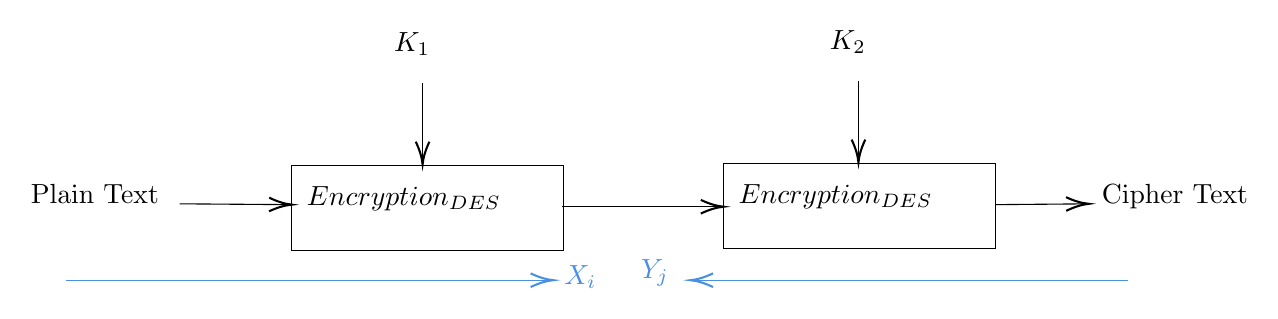
\begin{tikzpicture}[x=0.75pt,y=0.75pt,yscale=-1,xscale=1]
        
        \draw   (157,96) -- (288,96) -- (288,137) -- (157,137) -- cycle ;
        \draw   (365,95) -- (496,95) -- (496,136) -- (365,136) -- cycle ;
        \draw    (103,114.6) -- (155,114.99) ;
        \draw [shift={(157,115)}, rotate = 180.42] [color={rgb, 255:red, 0; green, 0; blue, 0 }  ][line width=0.75]    (10.93,-3.29) .. controls (6.95,-1.4) and (3.31,-0.3) .. (0,0) .. controls (3.31,0.3) and (6.95,1.4) .. (10.93,3.29)   ;
        \draw    (287,116) -- (363,116) ;
        \draw [shift={(365,116)}, rotate = 180] [color={rgb, 255:red, 0; green, 0; blue, 0 }  ][line width=0.75]    (10.93,-3.29) .. controls (6.95,-1.4) and (3.31,-0.3) .. (0,0) .. controls (3.31,0.3) and (6.95,1.4) .. (10.93,3.29)   ; 
        \draw    (496,115) -- (539,114.62) ;
        \draw [shift={(541,114.6)}, rotate = 179.49] [color={rgb, 255:red, 0; green, 0; blue, 0 }  ][line width=0.75]    (10.93,-3.29) .. controls (6.95,-1.4) and (3.31,-0.3) .. (0,0) .. controls (3.31,0.3) and (6.95,1.4) .. (10.93,3.29)   ; 
        \draw    (220,56.6) -- (220,93.6) ;
        \draw [shift={(220,95.6)}, rotate = 270] [color={rgb, 255:red, 0; green, 0; blue, 0 }  ][line width=0.75]    (10.93,-3.29) .. controls (6.95,-1.4) and (3.31,-0.3) .. (0,0) .. controls (3.31,0.3) and (6.95,1.4) .. (10.93,3.29)   ; 
        \draw    (430,55.6) -- (430,92.6) ;
        \draw [shift={(430,94.6)}, rotate = 270] [color={rgb, 255:red, 0; green, 0; blue, 0 }  ][line width=0.75]    (10.93,-3.29) .. controls (6.95,-1.4) and (3.31,-0.3) .. (0,0) .. controls (3.31,0.3) and (6.95,1.4) .. (10.93,3.29)   ; 
        \draw [color={rgb, 255:red, 74; green, 144; blue, 226 }  ,draw opacity=1 ]   (48,151.4) -- (281,151.4) ;
        \draw [shift={(283,151.4)}, rotate = 180] [color={rgb, 255:red, 74; green, 144; blue, 226 }  ,draw opacity=1 ][line width=0.75]    (10.93,-3.29) .. controls (6.95,-1.4) and (3.31,-0.3) .. (0,0) .. controls (3.31,0.3) and (6.95,1.4) .. (10.93,3.29)   ;
        \draw [color={rgb, 255:red, 74; green, 144; blue, 226 }  ,draw opacity=1 ]   (560,151.4) -- (351,151.4) ;
        \draw [shift={(349,151.4)}, rotate = 360] [color={rgb, 255:red, 74; green, 144; blue, 226 }  ,draw opacity=1 ][line width=0.75]    (10.93,-3.29) .. controls (6.95,-1.4) and (3.31,-0.3) .. (0,0) .. controls (3.31,0.3) and (6.95,1.4) .. (10.93,3.29)   ;
        
        \draw (163,105) node [anchor=north west][inner sep=0.75pt]   [align=left] {$Encryption_{DES}$};
        \draw (371,104) node [anchor=north west][inner sep=0.75pt]   [align=left] {$Encryption_{DES}$};
        \draw (30,104) node [anchor=north west][inner sep=0.75pt]   [align=left] {Plain Text};
        \draw (546,104) node [anchor=north west][inner sep=0.75pt]   [align=left] {Cipher Text};
        \draw (205,31) node [anchor=north west][inner sep=0.75pt]   [align=left] {$K_1$};
        \draw (415,30) node [anchor=north west][inner sep=0.75pt]   [align=left] {$K_2$};
        \draw (287,143) node [anchor=north west][inner sep=0.75pt]   [align=left] {\textcolor[rgb]{0.29,0.56,0.89}{$X_i$}};
        \draw (324,140) node [anchor=north west][inner sep=0.75pt]   [align=left] {\textcolor[rgb]{0.29,0.56,0.89}{$Y_j$}};
    \end{tikzpicture}
\end{center}
The key K will be concatenation of two 56-bit keys, i.e. $K = K_1 || K_2$. Let us consider the Known Plain Text Attack, i.e. the attacker knows the plaintext $M$ corresponding to cipher text $C$.
Therefore, 
\begin{center}
    $C = Enc(Enc(M, K_1), K_2)$\\
    \vspace{1mm}
    $keys = \{sk_1, sk_2,...., sk_{2^{56}}\}$
\end{center}
Since, the attacker has both, the cipher text as well as corresponding plain text. The attacker can perform the following:
\begin{center}
    $Enc(M, sk_i) = X_i$\\
    $Dec(C, sk_j) = Y_j$\\
\end{center}
The blue arrows in the above diagram represent the above steps. The attacker has performed encryption of the plain text in the forward direction using key $sk_i$, while decryption of cipher text using key $sk_j \neq sk_i$. Now,
\begin{center}
    if $X_i = Y_j \implies K_1 = sk_i$ and $K_2 = sk_j$
\end{center}
Two tables can be created, one that maps $sk_i$ with corresponding $X_i$, and other that maps $sk_j$ with corresponding $Y_j$. Now, we can do a lookup in these table, and where we find that $X_i = Y_j$, we get the secret key as:
\begin{center}
    $K = sk_i || sk_j$
\end{center}
Hence, Double DES will not provide any extra security over DES as the complexity will be more or less same (neglecting several smaller complexities). This is true, in general, for all the encryption algorithms.

\section{Triple Encryption of DES}
The standard mechanism to provide double security using DES is to use triple layer of encryption. The length of key in this remains 112-bit and it is a concatenation of two 56-bit keys. Let K be the key, then,
\begin{center}
    $K = K1 || K2$
\end{center}
\begin{center}
    \tikzset{every picture/.style={line width=0.75pt}}       
    
    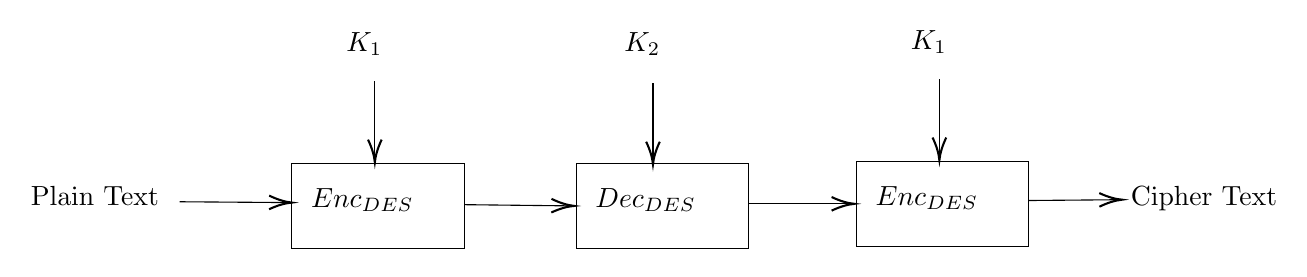
\begin{tikzpicture}[x=0.75pt,y=0.75pt,yscale=-1,xscale=1]
        \draw   (147,680.4) -- (230,680.4) -- (230,721.4) -- (147,721.4) -- cycle ;
        \draw    (93,699) -- (145,699.39) ;
        \draw [shift={(147,699.4)}, rotate = 180.42] [color={rgb, 255:red, 0; green, 0; blue, 0 }  ][line width=0.75]    (10.93,-3.29) .. controls (6.95,-1.4) and (3.31,-0.3) .. (0,0) .. controls (3.31,0.3) and (6.95,1.4) .. (10.93,3.29)   ;
        \draw    (230,700.4) -- (281,700.98) ;
        \draw [shift={(283,701)}, rotate = 180.65] [color={rgb, 255:red, 0; green, 0; blue, 0 }  ][line width=0.75]    (10.93,-3.29) .. controls (6.95,-1.4) and (3.31,-0.3) .. (0,0) .. controls (3.31,0.3) and (6.95,1.4) .. (10.93,3.29)   ;
        \draw    (502,698.4) -- (545,698.02) ;
        \draw [shift={(547,698)}, rotate = 179.49] [color={rgb, 255:red, 0; green, 0; blue, 0 }  ][line width=0.75]    (10.93,-3.29) .. controls (6.95,-1.4) and (3.31,-0.3) .. (0,0) .. controls (3.31,0.3) and (6.95,1.4) .. (10.93,3.29)   ; 
        \draw    (187,641) -- (187,678) ;
        \draw [shift={(187,680)}, rotate = 270] [color={rgb, 255:red, 0; green, 0; blue, 0 }  ][line width=0.75]    (10.93,-3.29) .. controls (6.95,-1.4) and (3.31,-0.3) .. (0,0) .. controls (3.31,0.3) and (6.95,1.4) .. (10.93,3.29)   ;
        \draw    (321,642) -- (321,679) ;
        \draw [shift={(321,681)}, rotate = 270] [color={rgb, 255:red, 0; green, 0; blue, 0 }  ][line width=0.75]    (10.93,-3.29) .. controls (6.95,-1.4) and (3.31,-0.3) .. (0,0) .. controls (3.31,0.3) and (6.95,1.4) .. (10.93,3.29)   ;
        \draw   (284,680.4) -- (367,680.4) -- (367,721.4) -- (284,721.4) -- cycle ;
        \draw   (419,679.4) -- (502,679.4) -- (502,720.4) -- (419,720.4) -- cycle ; 
        \draw    (367,700) -- (416,700) ;
        \draw [shift={(418,700)}, rotate = 180] [color={rgb, 255:red, 0; green, 0; blue, 0 }  ][line width=0.75]    (10.93,-3.29) .. controls (6.95,-1.4) and (3.31,-0.3) .. (0,0) .. controls (3.31,0.3) and (6.95,1.4) .. (10.93,3.29)   ;
        \draw    (459,640) -- (459,677) ;
        \draw [shift={(459,679)}, rotate = 270] [color={rgb, 255:red, 0; green, 0; blue, 0 }  ][line width=0.75]    (10.93,-3.29) .. controls (6.95,-1.4) and (3.31,-0.3) .. (0,0) .. controls (3.31,0.3) and (6.95,1.4) .. (10.93,3.29)   ;
        
        \draw (155,691.4) node [anchor=north west][inner sep=0.75pt]   [align=left] {$Enc_{DES}$};
        \draw (20,690.4) node [anchor=north west][inner sep=0.75pt]   [align=left] {Plain Text};
        \draw (550,690.4) node [anchor=north west][inner sep=0.75pt]   [align=left] {Cipher Text};
        \draw (172,616.4) node [anchor=north west][inner sep=0.75pt]   [align=left] {$K_1$};
        \draw (306,616.4) node [anchor=north west][inner sep=0.75pt]   [align=left] {$K_2$};
        \draw (292,691.4) node [anchor=north west][inner sep=0.75pt]   [align=left] {$Dec_{DES}$};
        \draw (427,690.4) node [anchor=north west][inner sep=0.75pt]   [align=left] {$Enc_{DES}$};
        \draw (444,615.4) node [anchor=north west][inner sep=0.75pt]   [align=left] {$K_1$};
    \end{tikzpicture}

    \textbf{Encryption}
    \vspace{3mm}
    
    \tikzset{every picture/.style={line width=0.75pt}}       
    
    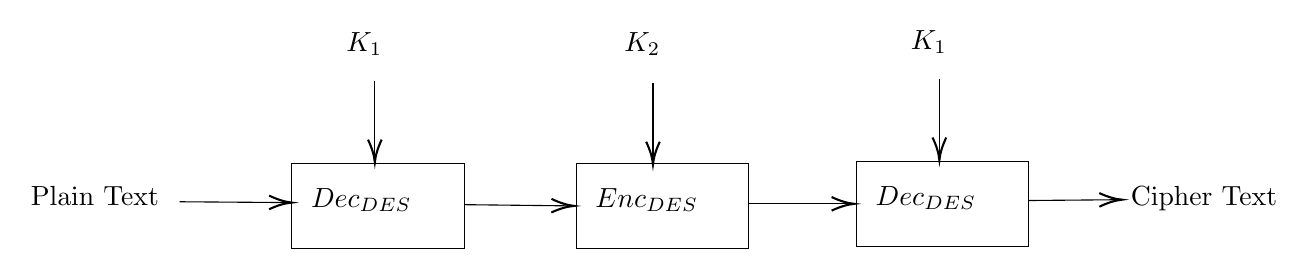
\begin{tikzpicture}[x=0.75pt,y=0.75pt,yscale=-1,xscale=1]
        \draw   (147,680.4) -- (230,680.4) -- (230,721.4) -- (147,721.4) -- cycle ;
        \draw    (93,699) -- (145,699.39) ;
        \draw [shift={(147,699.4)}, rotate = 180.42] [color={rgb, 255:red, 0; green, 0; blue, 0 }  ][line width=0.75]    (10.93,-3.29) .. controls (6.95,-1.4) and (3.31,-0.3) .. (0,0) .. controls (3.31,0.3) and (6.95,1.4) .. (10.93,3.29)   ;
        \draw    (230,700.4) -- (281,700.98) ;
        \draw [shift={(283,701)}, rotate = 180.65] [color={rgb, 255:red, 0; green, 0; blue, 0 }  ][line width=0.75]    (10.93,-3.29) .. controls (6.95,-1.4) and (3.31,-0.3) .. (0,0) .. controls (3.31,0.3) and (6.95,1.4) .. (10.93,3.29)   ;
        \draw    (502,698.4) -- (545,698.02) ;
        \draw [shift={(547,698)}, rotate = 179.49] [color={rgb, 255:red, 0; green, 0; blue, 0 }  ][line width=0.75]    (10.93,-3.29) .. controls (6.95,-1.4) and (3.31,-0.3) .. (0,0) .. controls (3.31,0.3) and (6.95,1.4) .. (10.93,3.29)   ; 
        \draw    (187,641) -- (187,678) ;
        \draw [shift={(187,680)}, rotate = 270] [color={rgb, 255:red, 0; green, 0; blue, 0 }  ][line width=0.75]    (10.93,-3.29) .. controls (6.95,-1.4) and (3.31,-0.3) .. (0,0) .. controls (3.31,0.3) and (6.95,1.4) .. (10.93,3.29)   ;
        \draw    (321,642) -- (321,679) ;
        \draw [shift={(321,681)}, rotate = 270] [color={rgb, 255:red, 0; green, 0; blue, 0 }  ][line width=0.75]    (10.93,-3.29) .. controls (6.95,-1.4) and (3.31,-0.3) .. (0,0) .. controls (3.31,0.3) and (6.95,1.4) .. (10.93,3.29)   ;
        \draw   (284,680.4) -- (367,680.4) -- (367,721.4) -- (284,721.4) -- cycle ;
        \draw   (419,679.4) -- (502,679.4) -- (502,720.4) -- (419,720.4) -- cycle ; 
        \draw    (367,700) -- (416,700) ;
        \draw [shift={(418,700)}, rotate = 180] [color={rgb, 255:red, 0; green, 0; blue, 0 }  ][line width=0.75]    (10.93,-3.29) .. controls (6.95,-1.4) and (3.31,-0.3) .. (0,0) .. controls (3.31,0.3) and (6.95,1.4) .. (10.93,3.29)   ;
        \draw    (459,640) -- (459,677) ;
        \draw [shift={(459,679)}, rotate = 270] [color={rgb, 255:red, 0; green, 0; blue, 0 }  ][line width=0.75]    (10.93,-3.29) .. controls (6.95,-1.4) and (3.31,-0.3) .. (0,0) .. controls (3.31,0.3) and (6.95,1.4) .. (10.93,3.29)   ;
        
        \draw (155,691.4) node [anchor=north west][inner sep=0.75pt]   [align=left] {$Dec_{DES}$};
        \draw (20,690.4) node [anchor=north west][inner sep=0.75pt]   [align=left] {Plain Text};
        \draw (550,690.4) node [anchor=north west][inner sep=0.75pt]   [align=left] {Cipher Text};
        \draw (172,616.4) node [anchor=north west][inner sep=0.75pt]   [align=left] {$K_1$};
        \draw (306,616.4) node [anchor=north west][inner sep=0.75pt]   [align=left] {$K_2$};
        \draw (292,691.4) node [anchor=north west][inner sep=0.75pt]   [align=left] {$Enc_{DES}$};
        \draw (427,690.4) node [anchor=north west][inner sep=0.75pt]   [align=left] {$Dec_{DES}$};
        \draw (444,615.4) node [anchor=north west][inner sep=0.75pt]   [align=left] {$K_1$};
    \end{tikzpicture}

    \textbf{Decryption}
\end{center}
different combinations such as EEE, EED, EDE etc. can be used. Consequently, the decryption will also have a different combination, where the E and D will be swapped, hence, DDD, DDE, DED etc. \\
\textbf{Note:} 
\begin{itemize}
    \item the key used in the middle function should be different than the key used in first and last function
    \item the key in first and last function must be same
\end{itemize}
\section{Advanced Encryption Standard}
DES design was initially kept secret but when it was made public, it was immediately broken. Thereafter, A lot of cryptographers around the world submitted their designs along with the implementation. One of the submission in the competition was $\emph{Rijndael}$. In the proposal, it was mentioned that the winner will be renamed as Advanced Encryption Standard. AES is unbreakable till date.\\
\vspace{3mm}
Before learning about the AES algorithm deeply, it is required to learn about certain mathematical structures.

\subsection{Mathematics Recall}
A binary operation $*$ on a set S is a mapping from $S \times S$ to S. It means $*$ is a rule which assigns to each ordered pair of elements from S to an element of S.
\begin{center}
    $*: S \times S \rightarrow S$ \\
    \vspace{1mm}
    if $*(a, b) = c$ and $a, b \in S \implies c \in S$\\
    \vspace{1mm}
    $*(b, a) = d \implies d \in S$
\end{center}
The ordering in the pair is important, hence, it is not necessary that $c = d$.

\subsubsection{Group}
A Group $(G, *)$ consists of a set $G$ and a binary operation $*$ on $G$ satisfying the following axioms:
\begin{enumerate}
    \item $*$ is associative on G, that is, $a * (b * c) = (a * b) * c$ $ \forall$ $ a,b,c \in G$
    \item There is an element $e \in G$ called the Identity Element, such that $a * e = a = e * a$ $\forall$ $a \in G$.
    \item For each $a \in G$, there exists an element $a^{-1} \in G$, called the inverse of $a$, such that $a * a^{-1} = e = a^{-1} * a$ $\forall$ $a \in G$. 
\end{enumerate}

\subsubsection{Abelian Group}
A group G is called an Abelian (or commutative) Group if $a * b = b * a$ $\forall$ $a,b \in G$.\\

\subsection{Examples}
\subsubsection{Example 1:}
Let,\\
$*$ : matrix multiplication over square matrices of order $n$ and\\
$M$: set of $n \times n$ matrices over $\mathbb{R}$.\\
Is $(M, *)$ a group?\\
\textbf{Solution:} We know that matrix multiplication is associative and hence $*$ is associative on $M$. Also, there always exist Identity Matrix $I_n$, such that $A * I_n = A = I_n * A$. However, 
\begin{center}
    $\forall$ $(A \in M) \nexists (A^{-1} \in M)$ such that $A * A^{-1} = I_n = A^{-1} * A$
\end{center}
The inverse of matrix doesn't exist if its determinant is equal to zero. Hence, $(M, *)$ is not a group.\\

\subsubsection{Example 2:}
Consider $M$ in the previous problem to be the set of all invertible square matrices and $*$ be the same. Clearly, $(M, *)$ will now be a group as non-invertible matrices do not belong to $M$. Is $(M, *)$ an Abelian Group?
\\
\textbf{Solution:} For a group to be an Abelian Group, it must be commutative over the set of elements. However, in general, matrix multiplication is not commutative, that is $A * B \neq B * A$. Hence, $(M, *)$ is not an Abelian Group.\\

\subsubsection{Example 3:}
$\mathbb{Z: }$ set of all integers and $+$ is addition operation. Is it a group?\\
\textbf{Solution:} We know that addition is associative, i.e, 
\begin{center}
    $a + (b + c) = (a + b) + c$\\
\end{center}
Also, $0 \in \mathbb{Z}$ is identity element such that:
\begin{center}
    $a + 0 = a = 0 + a$ $\forall$ $a \in \mathbb{Z}$
\end{center}
And, for each $a \in \mathbb{Z}$ $\exists (-a)$ such that $a + (-a) = 0 = (-a) + a$. Hence, $(\mathbb{Z}, +)$ is a group.\\
\vspace{3mm}
\textbf{Note:} $(\mathbb{Z}, -)$ is not a group as subtraction is not associative.\\

\subsubsection{Example 4:}
Consider the multiplication operation $\times$ on the set of integers $\mathbb{Z}$. Is it a group?\\
\textbf{Solution:} The multiplication operation is:
\begin{center}
    associative: $a \times (b \times c) = (a \times b) \times c$\\
    existence of identity element: $a \times 1 = a = 1 \times a$
\end{center}
However, inverse of a, that is, $a \times a^{-1} = 1 = a^{-1} \times a$ does not exist for multiplication operation on $\mathbb{Z}$. This is because, for multiplication operation $a^{-1} = \frac{1}{a} \notin \mathbb{Z}$. \\Hence, $(\mathbb{Z}, \times)$ is not a group.\\

\subsubsection{Example 5:}
set of all rational numbers and $\times$ is multiplication operation. Is $(\mathbb{Q}, \times)$ a group?\\
\textbf{Solution:} No, it is not a group. It satisfies all the other properties of a group but for $0 \in \mathbb{Q}$ inverse does not exist. Hence, $(\mathbb{Q}, \times)$ is not a group. However, if we consider the set $\mathbb{Q} - \{0\}$, then $(\mathbb{Q} - \{0\}, \times)$ is a group.\\
\vspace{3mm}
\textbf{Finite Group :}\\
If the number of elements in a set is finite, and $(G, *)$ is a group, then $(G, *)$ is a finite group.\\
\vspace{3mm}
\subsubsection{Example 6:}
Consider the set $\mathbb{Z}_n$ which contains integers from 0 to $n - 1$ (both inclusive) and the operation $+_n$ which means $x +_n y = (x + y) mod$ n. Is $(\mathbb{Z}_n, +_n)$ a group?\\
\textbf{Solution:} Let's check for each property one by one:\\
\begin{itemize}
    \item Associativity
    \begin{center}
        $(x +_n y) +_n z = (((x + y) mod n) + z) mod $ $n$\\
        \vspace{1mm}
        $\implies (x +_n y) +_n z = (x + y + z) mod $ $n$\\
        \vspace{1mm}
        $\implies (x +_n y) +_n z = (x + (y + z) mod $ $n) mod $ $n$\\
        \vspace{1mm}
        $\implies (x +_n y) +_n z = x +_n (y +_n z)$
    \end{center}
    Hence, $(\mathbb{Z}_n, +_n)$ is associative.

    \item Existence of Identity Element in $\mathbb{Z}_n$. Clearly, 0 is the identity element as :\\
    \begin{center}
        $x +_n 0 = x = 0 +_n x$.
    \end{center}

    \item Existence of inverse. Clearly, for $x \in \mathbb{Z}_n$, $n - x$ will be the inverse of $x$.
    \begin{center}
        $x +_n (n - x) = (x + n - x) mod$ $n = n$ $mod $ $n = 0$
    \end{center}
\end{itemize}
Hence, $(\mathbb{Z}_n, +_n)$ is a group. Moreover, it is an Abelian group.\\


\subsubsection{Example 7:}
Consider the set $(\mathbb{Z}_n - \{0\})$ and the operation $*_n$, i.e, $x *_n y = (x * y) mod$ $n$. Is $((\mathbb{Z}_n - \{0\}), *_n)$ a group?\\
\textbf{Solution:} It is easy to verify that the given operation is associative on the given set, and also it has an identity element equal to 1. Now, let us see for inverse. We know that for $x \in (\mathbb{Z}_n - \{0\})$, inverse $x^{-1}$ will be defined as:
\begin{center}
    $x *_n x^{-1} = 1 \implies x * x^{-1} \equiv 1$ $mod$ $n$
\end{center}
The $x^{-1}$ here is known as multiplicative inverse of $x$ under modulo $n$. We know that it exists only iff $gcd(x, n) = 1$. Hence, there may exist some $x$, for which $gcd(x, n) \neq 1$ and hence, $x^{-1}$ does not exist. Hence, $((\mathbb{Z}_n - \{0\}), *_n)$ is not a group.\\
\vspace{3mm}
Consider the set which has only those integers from 0 to n-1, which are co-prime to $n$. This set is usually denoted by $\mathbb{Z}_n^*$. The cardinality of this set can be calculated using the Euler's Totient Function $\phi(n)$.
\begin{center}
    $\mathbb{Z}_n^*$: $\{x \in \mathbb{Z}_n$ and $gcd(x,n) = 1\}$
\end{center}
Hence, $(\mathbb{Z}_n^*, *_n)$ is a group.
\end{document}